\documentclass[twofold]{article}

%\usepackage[sc]{mathpazo}
\usepackage{lmodern}
\usepackage{amssymb}
\usepackage[T1]{fontenc}
\linespread{1.05}
\usepackage{microtype}

\usepackage[english]{babel}

\usepackage[hmarginratio=1:1, top=32mm,columnsep=20pt]{geometry}
\usepackage[hang, small,labelfont=bf,up,textfont=it,up]{caption}
\usepackage{booktabs}

\usepackage{graphicx}
\usepackage{wrapfig}

\usepackage{mathtools}
\usepackage{amsthm}
\usepackage{abstract}
\renewcommand{\abstractnamefont}{\normalfont\bfseries}
\renewcommand{\abstracttextfont}{\normalfont\small}

\usepackage{lettrine}

%\usepackage{titlesec}
%\renewcommand\thesection{\Roman{section}}
%\renewcommand\thesubsection{\roman{subsection}}
%\titleformat{\section}[block]{\large\scshape\centering}{\thesection.}{1em}{}
%\titleformat{\subsection}[block]{\large}{\thesubsection.}{1em}{}

\usepackage{fancyhdr}
\pagestyle{fancy}
\fancyhead{}
\fancyfoot{}
\fancyhead[C]{Pranshu Gaba $\vert$ Summer Project 2017 $\vert$ Sr. No. 13718}
\fancyfoot[RO, LE]{\thepage}


\usepackage{titling}
\usepackage{hyperref}

\usepackage{mathtools}

%\setlength{\droptitle}{-6\baselineskip}
\pretitle{\begin{center}\huge\bfseries}
\posttitle{\end{center}}


\newcommand*\conj[1]{\overline{#1}}
\newcommand*\adj[1]{#1^*}
\newcommand*\norm[1]{\left \Vert #1 \right\Vert}
\newcommand*\abs[1]{\left \vert #1 \right\vert}
\newcommand*\trp[1]{#1^T}
\DeclareMathOperator{\Tr}{Tr}
\DeclarePairedDelimiterX{\inp}[2]{\langle }{\rangle }{#1, #2}


\theoremstyle{plain}
\newtheorem{theorem}{Theorem}
\newtheorem*{corollary}{Corollary}
\newtheorem*{lemma}{Lemma}

\theoremstyle{definition}
\newtheorem*{definition}{Definition}

\theoremstyle{remark}
\newtheorem*{remark}{Remark}

\author{%
\textsc{Pranshu Gaba}  \\[1ex]
\normalsize Indian Institute of Science, Bangalore \\
\normalsize \href{mailto:gabapranshu@iisc.ac.in}{gabapranshu@ug.iisc.in}}
\title{Hermitian Forms and Zeros of a Polynomial}
\date{\today}

\renewcommand{\maketitlehookd}{%

\begin{abstract}
We looked at various concepts in linear algebra such as norms, unitary matrices, and Hermitian matrices, and studied their applications. In particular, we examined the generalized Schur-Cohn theorem, which relates the number of roots of a polynomial lying within and without the unit circle with the parity of eigenvalues of a matrix formed by coefficients of the polynomial.

\[\textbf{Acknowledgements}\]

I am grateful to Prof. Tirthankar Bhattacharya for guiding me in this project, introducing me to new concepts and ideas in mathematics, challenging me to improve myself, and  for making this an enriching experience altogether.
\end{abstract}
}

\begin{document}
\maketitle

\section{Introduction}

%\lettrine[nindent=0em,lines=2]{I}

In this paper we see the properties of Hermitian matrices, which are very useful and interesting. We also see and prove the Schur-Cohn theorem to find the number of roots of a polynomial lying within the unit circle. 

There are many ways to locate the roots of a polynomial. The Schur-Cohn theorem shows a surprising connection between linear algebra and roots of a polynomial. It will be used to find out how many roots of the polynomial lie inside and outside the unit circle.

First we will define some basic terms that will be used ahead in the paper.

\section{Definitions}



\subsection{Norm of a matrix}

\subsubsection{Operator norm}
Given \(A \in \mathbb{M}_n\) (the set of \(n \times n\) square matrices with complex elements), the operator norm of \(A\), denoted by \(\norm{A}\), is defined as \[\norm{A} =\displaystyle \sup _{x \neq 0} \frac{\norm{Ax}}{\norm{x}} = \sup_{\norm{x} = 1} \norm{Ax} \]

\begin{theorem} The operator norm satisfies the triangle inequality \(\norm{A + B} \leq \norm{A} + \norm{B}\). \end{theorem}
\begin{proof} \begin{equation*} \begin{split}
\norm{A + B}  = \sup _{x \ne 0} \frac{\norm{(A + B) x}}{\norm{x}} & \le \sup_{x \ne 0} \frac{\norm{Ax} +\norm{Bx}}{\norm{x}} \\
& \le \sup_{x \ne 0} \frac{\norm{Ax}}{\norm{x}} + \sup_{x \ne 0} \frac{\norm{Bx}}{\norm{x}} = \norm{A} + \norm{B}
\end{split} \end{equation*} \end{proof}

\begin{theorem}\label{submulti} The operator norm is submultiplicative,  \(\norm{AB} \le \norm{A} \norm{B}\) for all square matrices \(A, B \in \mathbb{M}_n\). \end{theorem}
\begin{proof} \begin{equation*} \begin{split}
 \norm{AB} & = \sup_{x \ne 0} \frac{\norm{ABx}}{\norm{x}}\\
 & = \sup_{Bx \ne 0} \frac{\norm{ABx}}{\norm{x}} \\
& = \sup_{Bx \ne 0} \frac{\norm{ABx}}{\norm{Bx}} \frac{\norm{Bx}}{\norm{x}} \\
& \le \sup_{y \ne 0} \frac{\norm{Ay}}{\norm{y}} \sup_{x \ne 0} \frac{\norm{Bx}}{\norm{x}} = \norm{A} \norm{B} 
\end{split} \end{equation*}\end{proof}

\subsubsection{Hilbert-Schmidt norm}

The Hilbert-Schmidt norm of matrix \(A\), denoted by \(\norm{A}_2\),  is defined as the square root of sum of squares of all entries in \(A\). 

 \[\norm{A}_2 = \left( \sum_{i, j} \abs{a_{ij}}^2 \right) ^{1/2}\]


\begin{theorem} The operator norm is always less than or equal to the Hilbert-Schmidt norm. \end{theorem}
\begin{proof}
 \begin{equation*} \begin{split} 
\norm{Ax}^2 & = \sum_{i = 1} ^ n \abs{\sum_{j = 1} ^ n a_{ij} x_j}^2 \\
& \le  \sum_{i = 1} ^ n \left( \sum_{j = 1} ^ n \abs{a_{ij}} \abs{ x_j}\right) ^2 \\
& \le \left( \sum_{i = 1}^n \sum_{j = 1}^n \abs{a_{ij}}^2\right) \left( \sum_{j=1}^n \abs{x_j}^2 \right)  = \left( \sum_{i, j} \abs{a_{ij}}^2 \right) \norm{x}^2
\end{split}
\end{equation*} 
Therefore \(\displaystyle \frac{\norm{Ax}}{\norm{x}} \le \left( \sum_{i, j} \abs{a_{ij}}^2 \right) ^{1/2}\), which is equivalent to \(\norm{A} \le \norm{A}_2\).
\end{proof}


\subsection{Inner product}

The inner product is a binary operator on two vectors \(\inp{\cdot}{\cdot} \colon V  \times  V \to \mathbb{C}\). It  satisfies the following conditions for all \(x, y, z \in V\) and \(a \in \mathbb{C}\):

\begin{itemize}
\item It is linear in the first term. 

\(\quad \inp{ax}{y} = a \inp{x}{y}\)
 
\(\quad \inp{x + y}{z} = \inp{x}{z} + \inp{y}{z}\)

\item It becomes its complex conjugate when the arguments are reversed.

\(\quad \inp{x}{y} = \conj{\inp{y}{x}}\)

\item Inner product of a vector with itself is non-negative. 

\(\quad \inp{x}{x} \ge 0\). Here equality is achieved if and only if \(x = 0\).
\end{itemize}

For vectors on \(\mathbb{C}^n\), the inner product \(\inp{x}{y}\) is defined as \(\trp{x} \conj{y}\), the vector multiplication of the transpose of the first term with the complex conjugate of the second term. This definition satisfies all the above mentioned conditions.

\subsection{Positive Definite Matrix}

A matrix \(A\in \mathbb{M}_n\) that satisfies \(\inp{Ax}{x} \ge 0\) for all \(x \in \mathbb{C}^n\) is called a {\em positive semidefinite matrix} and is denoted as \(A \ge 0\). If the inequality is strict, \(\inp{Ax}{x} > 0\), then \(A\) is called a {\em positive definite matrix}, and it is denoted as \(A > 0\). 

For two matrices \(A, B \in \mathbb{M}_n\), \(A \le B\) denotes \(B - A\) is positive semidefinite. As a result, \(\inp{(B - A)x}{x} \ge 0\), or \(\inp{Ax}{x} \le \inp{Bx}{x}\) for all \(x\).

\begin{theorem} Let \(A \in \mathbb{M}_n\) be a positive semidefinite matrix. Then all eigenvalues of \(A\) are non-negative. \end{theorem}
\begin{proof} Let \(\lambda_1, \lambda_2, \ldots , \lambda_n\) be the eigenvalues of \(A\), and let \(x_1, x_2, \ldots , x_n\) be the corresponding eigenvectors, that is: \(Ax_i = \lambda x_i\). 

 For any eigenvector \(x_i\), the inner product \(\inp{Ax_i}{x_i} = \inp{\lambda_i x_i}{x_i}\). Since \(\lambda_i\) is a scalar, it can come out of the inner product, so  \( \inp{\lambda_i x_i}{x_i}  = \lambda_i \inp{x_i}{x_i}\). We get

\[\lambda_i = \frac{\inp{Ax_i}{x_i}}{\inp{x_i}{x_i}}\]

Here \(\inp{Ax_i}{x_i} \) is non-negative because \(A\) is positive semidefinite, and \(\inp{x_i}{x_i}\) is positive by definition of inner product. Hence \(\lambda_i \ge 0\); all eigenvalues of \(A\) are non-negative. \end{proof}


\subsection{Adjoint}

Let \(A \in \mathbb{M}_n\). The adjoint of matrix \(A\), denoted by \(\adj{A}\), is the matrix that  satisfies \(\inp{\adj{A}x}{y} = \inp{x}{Ay}\). The adjoint of a matrix, \(\adj{A}\), like \(A\), represents a linear transformation on \(\mathbb{C}^n\).

\begin{theorem} The adjoint of a matrix is obtained by taking the complex conjugate of every element, followed by transposing the matrix. \end{theorem}

\begin{proof} Using properties of inner product on \(\mathbb{C}^n\),
\begin{equation*} \begin{split}
\inp{\adj{A}x}{y} & = \trp{(\adj{A}x)} \conj{y}  \\
& = \trp{x} \trp{(\adj{A})} \conj{y}\\
= \inp{x}{Ay} & = \trp{x} \conj{Ay} 
\end{split} \end{equation*}

Therefore \(\trp{(\adj{A})} = \conj{A}\), or \(\adj{A} = \trp{(\conj{A})}\). \end{proof}

\begin{remark} The adjoint of the adjoint of a matrix is the original matrix itself, \(\adj{(\adj{A})} = A\). \end{remark}




\begin{theorem} The norm of a matrix is equal to the norm of its adjoint. \(\norm{A} = \norm{\adj{A}}\) \end{theorem}
\begin{proof}
\[ \norm{A}^2   = \sup_{\norm{x} = 1} \norm{Ax}^2  = \sup_{\norm{x} = 1} \inp{Ax}{Ax}  = \sup_{\norm{x} = 1} \inp{\adj{A} A x}{x}  = \norm{\adj{A} A} \]

\[ \norm{\adj{A}}^2   = \sup_{\norm{x} = 1} \norm{\adj{A} x}^2  = \sup_{\norm{x} = 1} \inp{\adj{A}x}{\adj{A}x}  = \sup_{\norm{x} = 1} \inp{A \adj{A} x}{x}  = \norm{A \adj{A}} \le \norm{A} \norm{\adj{A}}\]

However, using  Theorem \ref{submulti}, we get  \(\norm{\adj{A} A} \le \norm{\adj{A}} \norm{A}\) in the first equation. Hence, \(\norm{A}^2 \le \norm{\adj{A}} \norm{A}\), which implies  \(\norm{A} \le \norm{\adj{A}}\). Similarly, in the second equation we get \(\norm{\adj{A}} \le \norm{A}\). 

Since both these inequalities are true, it necessarily means that \(\norm{A} = \norm{\adj{A}}\).
\end{proof}

\begin{theorem}\label{pdm} \(\adj{A} A\) and \(A \adj{A}\) are positive semidefinite for all \(A \in \mathbb{M}_n\). \end{theorem}
\begin{proof} \(\inp{\adj{A} A x}{ x} = \inp{Ax}{Ax} = \norm{Ax}^2 \ge 0\)\end{proof}

\subsection{Unitary Matrix}

A square matrix \(U\) that satisfies \(\adj{U} U = I\) is called a unitary matrix.

\begin{theorem} The columns of a unitary matrix \(U\) form an orthonormal basis. \end{theorem}
\begin{proof}  Let \(u_i\) be the \(i^\text{th}\) column of \(U\). Then \(U = \begin{bmatrix} u_1 & u_2 & u_3 & \cdots & u_n \end{bmatrix}\) and \(\adj{U} = \begin{bmatrix} \adj{u_1} \\ \adj{u_2} \\ \adj{u_3} \\ \vdots \\ \adj{u_n} \end{bmatrix} \). 

Using the fact that \(U\) is a unitary matrix, \(\adj{U} U = I\):

\[  \begin{bmatrix} \adj{u_1} \\ \adj{u_2} \\ \adj{u_3} \\ \vdots \\ \adj{u_n} \end{bmatrix} \begin{bmatrix} u_1 & u_2 & u_3 & \cdots & u_n \end{bmatrix} = \begin{bmatrix} 1 & 0 & 0 & \cdots & 0 \\
0 & 1 & 0 & \cdots & 0 \\
0 & 0 & 1 & \cdots & 0 \\
\vdots & \vdots & \vdots & \ddots & \vdots \\
0 & 0 & 0 & \cdots & 1\end{bmatrix}\]

We see that \(\adj{u_i} u_j = \inp{u_i}{u_j} = \delta_{ij}\). Here \(\delta_{ij}\) is the Kronecker Delta function which is defined as

\[\delta_{ij} = \begin{cases} 
0 & \text{if } i \ne j \\
1 & \text{if } i = j \end{cases}
 \]


Each column has norm 1 since \(\inp{u_i}{u_i}= \norm{u_i}^2  =1\), and any two columns are orthogonal \(\inp{u_i}{u_j} = 0\). Hence the column vectors \(u_1, u_2, \ldots , u_n\) of a unitary matrix form an orthonormal basis.
    \end{proof}


\begin{theorem} A unitary matrix preserves inner product: \(\inp{Ux}{Uy} = \inp{x}{y}\) for all  \(x, y \in \mathbb{C}_n\) . \end{theorem}

\begin{proof} \(\inp{x}{y} = \inp{Ix}{y} = \inp{\adj{U}U x}{y} = \inp{Ux}{Uy}\) \end{proof}

\subsection{Trace}
The trace of matrix \(A\) is the sum of the diagonal elements of the matrix.

\[\Tr(A) = \sum_{i=1} ^n a_{ii} = \sum_{i=1} ^n \inp{Ae_i}{ e_i}\]

\begin{remark}Here \(a_{ij}\) denotes the element in the \(i^{\text{th}}\) row and \(j^{\text{th}}\) column. \(e_i\) denotes the \(i^{\text{th}}\) standard basis vector. Note that \(a_{ij} = \inp{e_i}{e_j}\).\end{remark}

\begin{theorem}The trace of \(\adj{A}A\) is equal to the square of the Hilbert-Schmidt norm of \(A\). \[\Tr( \adj{A} A ) = \norm{A}_2^2\]\end{theorem}
\begin{proof}
The sum of diagonal elements of \(\adj{A} A\) is
 \begin{equation*} \begin{split} 
\Tr(\adj{A} A) & = \sum_{i=1}^n \inp{\adj{A}A e_i}{e_i} \\
 & = \sum_{i=1} ^n \inp{Ae_i}{Ae_i} \\
& = \sum_{i=1} ^n \norm{Ae_i}^2 \\
& = \sum_{i=1} ^n \sum_{j=1} ^n \abs{a_{ji}}^2  = \norm{A}^2_2
\end{split} \end{equation*}
 \end{proof}

\subsection{Hermitian Matrix}
A matrix that satisfies \(A = \adj{A}\) is called a Hermitian matrix (or a self-adjoint matrix). 

\begin{theorem} \label{herm_eig_real} Let \(A \in \mathbb{M}_n\) be a Hermitian matrix. Then all eigenvalues of \(A\) are real. \end{theorem}

\begin{proof}
Let \(v\) be an eigenvector of a matrix \(A\), and let \(\lambda\) be the corresponding eigenvalue. Then \(Av = \lambda v\). 

\[ \lambda\inp{v}{v} = \inp{\lambda v}{v} =  \inp{Av}{v} = \inp{v}{\adj{A}v} = \inp{v}{Av} = \inp{v}{\lambda v} = \conj{\lambda} \inp{v}{v}\]

This implies \(\lambda = \conj{\lambda}\) for all \(v\). Hence, \(\lambda\) is real. All eigenvalues of a Hermitian matrix are real.
 \end{proof}



\begin{theorem} Eigenvectors corresponding to distinct eigenvalues are orthogonal.\end{theorem}

\begin{proof} Suppose \(\lambda\) and \(\mu\) are distinct eigenvalues of \(A\). Suppose the corresponding eigenvectors are \(u\) and \(v\) respectively. We have \(Au = \lambda u\) and \(Av = \mu v\). Since \(A\) is Hermitian, 

\[ \lambda \inp{u}{v} = \inp{\lambda u}{v} = \inp{A u}{v} = \inp{u}{Av} = \inp{u}{\mu v} = \mu \inp{u}{v} \]

Since \(\lambda \ne \mu\), \(\inp{u}{v}\) must be zero. Eigenvectors \(u\) and \(v\) are orthogonal.

\end{proof}



A diagonal matrix is a matrix whose non-diagonal entries are all zero. \(a_{ij} = 0\) if \(i \ne j\)

\begin{theorem}[Spectral theorem]  For every Hermitian matrix \(A\), there exists a unitary matrix \(U\) such that \(A = U \Lambda \adj{U}\), where \(\Lambda\) is the diagonal matrix \(\begin{bmatrix}
\lambda_1 & 0 & 0 & \cdots & 0\\
0 & \lambda_2 & 0 & \cdots & 0\\
0 & 0 & \lambda_3 & \cdots & 0\\
\vdots & \vdots & \vdots & \ddots & \vdots \\
0 & 0 & 0 & \cdots & \lambda_n \end{bmatrix}\) containing eigenvalues of \(A\). \end{theorem}

\begin{proof} 
The matrix \(A\) is a linear transformation \(T\) with respect to the standard basis \(I\). The matrix \(U\) is a unitary matrix, so its columns \(u_1, u_2, \ldots , u_n\) form an orthonormal basis for \(\Lambda\). Since \(U\) is a unitary vector, \(\adj{U} = U^{-1}\). This means \(\Lambda\) is the matrix of the same transformation \(T\) with respect to a different basis \(U\), and that \(A\) and \(\Lambda\) have the same eigenvalues.


Start with any eigenvalue \(\lambda_1\) of \(A\). Let \(x_1\) be a unit eigenvector corresponding to \(\lambda_1\).

The basis transforms from \(x_i \mapsto \adj{U}x_i\)

\(AU = U\Lambda\)

% finish the proof
\end{proof}


Let \(A\) be Hermitian. Its eigenvalues are \(\lambda_1 \le \lambda_2 \le \cdots \le \lambda_n\). Using spectral theorem, 

\[\frac{\inp{Ax}{x}}{\inp{x}{x}}  = \frac{\inp{U\Lambda \adj{U}x}{x}}{\inp{x}{x}} = \frac{\inp{\Lambda y}{y}}{\inp{y}{y}} = \frac{\sum \lambda_i \abs{y_i}^2}{\sum \abs{y_i}^2}\]

\(\{x \in \mathbb{C}^n : x \ne 0\} = \{y \in \mathbb{C}^n : y = \adj{U} x \text{ for } x \ne 0 \} \) 


We get the following inequality. 

\[\lambda_1 = \lambda_1 \frac{\sum \abs{y_i}^2}{\sum \abs{y_i}^2} \le \frac{\sum \lambda_i \abs{y_i}^2}{\sum \abs{y_i}^2} \le  \lambda_n \frac{\sum \abs{y_i}^2}{\sum \abs{y_i}^2} = \lambda_n\]

Therefore \[ \lambda_1 \le \frac{\inp{Ax}{x}}{\inp{x}{x}} \le \lambda_n\]

\[\lambda_1 = \inf _{x \ne 0} \frac{\inp{Ax}{x}}{\inp{x}{x}}, \quad \lambda_n = \sup_{x \ne 0} \frac{\inp{Ax}{x}}{\inp{x}{x}}\]




\begin{theorem} \label{hermit_real} If \(A \in \mathbb{M}_n\) is Hermitian, then \(\inp{Ax}{x}\) is real for all \(x\). \end{theorem}
\begin{proof} \(\inp{Ax}{x} = \inp{x}{\adj{A}x} = \inp{x}{Ax} = \conj{\inp{Ax}{x}}\). \end{proof}

The converse of this theorem is also true.

\begin{theorem}[Converse of Theorem \ref{hermit_real}]\label{eig_real_herm} If \(A \in \mathbb{M}_n\) and \(\inp{Ax}{x} \in \mathbb{R}\) for every \(x \in \mathbb{C}_n\), then \(A\) is a Hermitian matrix. \end{theorem}

\begin{proof} Let \(\alpha \in \mathbb{C}\) and \(h, g \in \mathbb{C}^n\). Then
\[\inp{A(h + \alpha g)}{h + \alpha g} = \inp{Ah}{h} + \alpha \inp{Ag}{h} + \conj{\alpha} \inp{Ah}{g} + \abs{\alpha}^2 \inp{Ag}{g} \]

The first and the last terms \(\inp{Ah}{h}\) and \(\abs{\alpha}^2 \inp{Ag}{g}\) are both real. We now look at the sum of second and third terms:
\[\alpha \inp{Ag}{h} + \conj{\alpha} \inp{Ah}{g} = \conj{\alpha} \inp{h}{Ag} + \alpha \inp{g}{Ah} \]

We can substitute values of \(\alpha = 1\) and \(\alpha = i\)  in this equation to get a system of linear equations. 
\begin{equation*}
\begin{aligned}
\inp{Ag}{h}  + \inp{Ah}{g} & =  \inp{h}{Ag}  + \inp{g}{Ah} \\
i \inp{Ag}{h}  - i \inp{Ah}{g}  & = -i \inp{h}{Ag} +  i \inp{g}{Ah} 
\end{aligned}
\end{equation*}

Solving this system gives us \(\inp{Ag}{h} = \inp{g}{Ah}\), which is equal to \(\inp{\adj{A}g}{h}\). Hence \(Ag = \adj{A}g\) for all \(g\), and \(A = \adj{A}\). We see that \(A\) is a Hermitian matrix.
\end{proof}

\begin{corollary}Every positive semidefinite matrix \(A \in \mathbb{M}_n\) is Hermitian.\end{corollary}
\begin{proof} \(A\) is a positive semidefinite matrix, so \(\inp{Ax}{x} \ge 0 \),  so \(\inp{Ax}{x} \in \mathbb{R}\) for all \(x\). By Theorem \ref{eig_real_herm}, \(A\) is Hermitian. \end{proof}

\begin{theorem}\label{norm_herm} If \(A\) is Hermitian, then \(\norm{A} = \sup\{\abs{\inp{Ah}{h}} : \norm{h} = 1\}\).\end{theorem}
\begin{proof} By Cauchy Schwarz, \(\norm{Ah}\norm{h} \ge \abs{\inp{Ah}{h}}\). For \(\norm{h} =1\), we have  \(\norm{A} \ge \abs{\inp{Ah}{h}}\). Now we will prove the reverse inequality. 

Let \(M = \sup \{\abs{\inp{Ah}{h}} : \norm{h} = 1 \}\). If \(h, g \in \mathbb{C}^n\) with \(\norm{h} = \norm{g} = 1\), then

\begin{equation*} \begin{split}
\inp{A (h \pm g)}{h\pm g} & = \inp{Ah}{h} \pm \inp{Ah}{g} \pm \inp{Ag}{h} + \inp{Ag}{g} \\
& = \inp{Ah}{h} \pm \inp{Ah}{g} \pm \inp{g}{Ah} + \inp{Ag}{g} \\
& = \inp{Ah}{h} \pm 2 \text{Re}\inp{Ah}{g} + \inp{Ag}{g} \\
\end{split} \end{equation*}

From this, we get a bound on \(\mathrm{Re}\inp{Ah}{g}\):
\begin{equation*} \begin{split}
4\mathrm{Re} \inp{Ah}{g} &= \inp{A(h+g)}{h+g} - \inp{A(h-g)}{h-g} \\
& \le \abs{\inp{A(h+g)}{h+g}} + \abs{\inp{A(h-g)}{h-g}} \\
& \le \abs{\inp{A \frac{h+g}{\norm{h+g}}}{\frac{h+g}{\norm{h+g}}}} \norm{h + g}^2 + \abs{\inp{A \frac{h-g}{\norm{h-g}}}{\frac{h-g}{\norm{h-g}}}} \norm{h - g}^2\\
& \le M (\norm{h + g}^2 + \norm{h-g}^2) \\
& = M (2 \norm{h}^2 + 2 \norm{g}^2) = 4M 
\end{split} \end{equation*}


We get \(\text{Re} \inp{Ah}{g} \le M\) for any \(h, g \in \mathbb{C}^n\) with \(\norm{h} = \norm{g} = 1\). 

If \(\inp{Ah}{g}\) is not real, then we can write it as  \(\inp{Ah}{g} = e^{i \theta} \abs{\inp{Ah}{g}}\). We get \(\abs{\inp{Ah}{g}} = e^{-i \theta} \inp{Ah}{g}\) is real, and is equal to \(\inp{A e^{- i\theta}h}{g}\). Since \(\norm{e^{-i\theta} h}= 1\), the above inequality still holds:
 \[\abs{\inp{Ah}{g}} = \inp{Ae^{-i\theta}h}{g} =  \text{Re} \inp{Ae^{-i\theta}h}{g} \le M\]

We also have the following relation
 \[\norm{A} = \sup_{\norm{h} =1} \norm{Ah} = \sup_{\norm{h = 1}} \sup_{\norm{g} = 1} \abs{\inp{Ah}{g}} \]

Therefore \(\abs{\inp{Ah}{g}} \le M\)  implies \(\norm{A} \le M\). Since \(\norm{A} \ge M\) and \(\norm{A} \le M\) both hold true, it means that \(\norm{A} = M = \sup \{ \abs{\inp{Ah}{h}} : \norm{h} = 1 \}\).
\end{proof}

\begin{corollary} If \(\inp{Ax}{x} = 0\) for all \(x\), then \(A = 0\).\end{corollary}
\begin{proof} Since \(\inp{Ax}{x} = 0\) for all \(x\), we have \(\sup \abs{\inp{Ax}{x}} = 0\). By Theorem \ref{norm_herm},\( \norm{A} = 0 \). This is true only when \(A = 0\).\end{proof}


\begin{corollary} If \(A \ge 0\), then \(\displaystyle \norm{A} = \sup _{\norm{x} = 1} \inp{Ax}{x}\) \end{corollary}
\begin{proof}   By the Corollary in Theorem \ref{eig_real_herm}, every positive semidefinite matrix is Hermitian, and for a positive semidefinite matrix, \(\abs{\inp{Ax}{x}} = \inp{Ax}{x}\). Hence, \(\norm{A} = \displaystyle \sup_{\norm{x} = 1} \inp{Ax}{x}\) \end{proof}



\begin{theorem}[Courant-Fischer] Let \(A \in \mathbb{M}_n\) be a Hermitian matrix with eigenvalues \(\lambda_1 \le \lambda_2 \le \lambda_3 \le \cdots \le \lambda_n\).  Then 
\begin{equation*}\begin{split}
 \lambda_k &= \min_{w_1, \ldots , w_{n-k} \in \mathbb{C}^n} \max_{\substack{x \neq 0, x\in \mathbb{C}^n \\ x \perp w_1, \ldots , w_{n-k}}} \frac{\inp{Ax}{x}}{\inp{x}{x}} \\
& = \max_{w_1, \ldots , w_{k -1} \in \mathbb{C}^n} \min_{\substack{x \neq 0, x\in \mathbb{C}^n \\ x \perp w_1, \ldots , w_{k - 1}}} \frac{\inp{Ax}{x}}{\inp{x}{x}}
\end{split} \end{equation*}
 \end{theorem}


\begin{proof} 

 If \(x \neq 0\), then \[\frac{\inp{Ax}{x}}{\inp{x}{x}} = \frac{\inp{U \Lambda \adj{U} x}{x}}{\inp{\adj{U} x}{ \adj{U} x}} =  \frac{\inp{\Lambda \adj{U} x}{ \adj{U} x}}{\inp{\adj{U}x}{\adj{U}x}}\]

Since \(U\) is a unitary matrix, its columns form an orthonormal basis.  \(\adj{U}x\) spans and \( \{ \adj{U} x \mid x \neq 0\}  = \{x \in \mathbb{C}^n \mid x \ne 0 \}\) 



Thus if \(w_1, \ldots , w_{n-k}\) are given, then 

\begin{equation*} \begin{split}
\sup_{\substack{x \neq 0 \\ x \perp w_1, \ldots, \ w_{n-k}}} \frac{\inp{Ax}{x}}{\inp{x}{x}} & = \sup_{\substack{y \neq 0 \\ y \perp \adj{U} w_1, \ldots ,\ \adj{U} w_{n-k}}} \frac{\inp{\Lambda y}{y}}{\inp{y}{y}} \\
%\textrm{x \perp w if and only if y \perp \adj{U} \omega.} \\
&  = \sup_{\substack{\inp{y}{y} = 1 \\ y \perp \adj{U} w_1, \ \ldots , \ \adj{U}w_{n-k}}} \sum_{i = 1}^n \lambda_i \abs{y_i}^2 \\
&  \ge \sup_{\substack{\inp{y}{y} = 1 \\ y \perp \adj{U} w_1, \ \ldots , \ \adj{U} w_{n-k} \\ y_1 = y_2 = \cdots = y_{k-1} = 0 }} \sum_{i = 1}^n \lambda_i \abs{x_i}^2 \\
&  = \sup_{\substack{\inp{y}{y} = 1 \\ y \perp \adj{U} w_1, \ \ldots , \ \adj{U} w_{n-k} \\ y_1 = y_2 = \cdots = y_{k-1} = 0 }} \sum_{i = k}^n \lambda_i \abs{y_i}^2 \\
&  \ge \lambda_k 
\end{split} \end{equation*}


Let \(w_1 = x_n , \ w_2 = x_{n-1}, \ \ldots , \ w_{n-k} = x_{k + 1}\)

If \(x\perp w_i\), as above, then \(x = \sum_{i = 1} ^k c_i x_i\). 

\begin{equation*} \begin{split}
\inp{Ax}{x} & = \inp{A \sum_{i = 1} ^ n c_i x_i}{ \sum_{i = 1} ^n c_i x_i} \\
&  = \inp{\sum_{i = 1} ^n c_i \lambda_i x_i}{\sum_{i = 1} ^n c_i x_i}\\
& = \sum_{i = 1} ^ k \lambda_i \abs{c_i}^2 \\
&  \le \lambda_k \sum_{i = 1} ^{k} \abs{c_i}^2
\end{split} \end{equation*}
\end{proof}


\subsection{Projectors}
A matrix \(P\) is a projector if \(P^2 = P\) and \(\adj{P} = P\)

\begin{theorem} There exists a subspace \(M\) of \(\mathbb{C}^n\) such that 

\[\begin{cases}
Pm = m & \forall m \in M \\
Px = 0 & \forall x \in M^\perp 
\end{cases}\] 
\end{theorem}
\begin{proof}  \(\mathrm{range}(P)= M\) and \(\mathrm{range}(I - P) = M^\perp\) satisfy the above properties. These subspaces are orthogonal. Let \(Pv \in M\), \(w - Pw \in M^\perp\). 
\[\inp{w - Pw}{Pv} = \inp{w}{Pv} - \inp{Pw}{Pv} = \inp{w}{Pv} - \inp{w}{\adj{P}Pv} = \inp{w}{Pv} - \inp{w}{P^2v} = \inp{w}{Pv} - \inp{w}{Pv} = 0\]

Let \(m \in \mathrm{range}(P)\), that is, \(m= Pv\) for some \(v \in \mathbb{C}^n\). Then \(Pm = P^2 v = Pv = m\). 

Now let \(x \in \mathrm{range}(I - P)\), that is, \(x = (I - P) = v - Pv\) for some \(v \in \mathbb{C}^n\). \(Px = Pv - P^2v = Pv - Pv = 0\).
%frame the arguments better
 \end{proof}

\subsection{Shift Matrix}
Let \(S\), the {\em shift matrix},  be the \(n \times n\) square matrix \( \begin{bmatrix} 
0 & 1 & 0 & \cdots & 0 \\
0 & 0 & 1 & \cdots & 0 \\
\vdots & \vdots & \vdots &\ddots & \vdots \\
0 & 0 & 0 &\cdots & 1 \\
0 & 0 & 0 & \cdots & 0 \\ 
\end{bmatrix}\). 

 \begin{remark} \(S\) is a nilpotent matrix of order \(n\), i.e. \(S^n\) is a zero matrix. \end{remark}

% \begin{remark} \(\norm{S} < 1\) \end{remark}

The following matrices will be useful in proving the Schur-Cohn theorem. Note that \(I - \adj{S} S = e_1 \adj{e_1}\) is a projector matrix.
\[\adj{S} =  \begin{bmatrix} 
0 & 0 & \cdots & 0 & 0 \\
1 & 0 & \cdots & 0 & 0 \\
0 & 1 & \cdots & 0 & 0 \\
\vdots & \vdots & \ddots &\vdots & \vdots \\
0 & 0 & \cdots & 1 & 0 \\ 
\end{bmatrix}, \quad 
\adj{S} S  =  \begin{bmatrix} 
0 & 0 & 0 & \cdots & 0 \\
0 & 1 & 0 & \cdots & 0 \\
0 & 0 & 1 & \cdots & 0 \\
\vdots & \vdots & \vdots & \ddots & \vdots \\
0 & 0 & 0 & \cdots & 1
\end{bmatrix}, \quad 
 I - \adj{S} S =  \begin{bmatrix} 
1 & 0 & \cdots & 0 & 0 \\
0 & 0 & \cdots & 0 & 0 \\
\vdots & \vdots & \ddots &\vdots & \vdots \\
0 & 0 & \cdots & 0 & 0 \\ 
0 & 0 & \cdots & 0 & 0
\end{bmatrix}\]



\section{Schur-Cohn Theorem}

\subsection{Theorem}
For any polynomial \[p(z) = a_0 z^n + a_1z^{n-1} + a_2 z^{n-2} + \cdots +  a_{n-1} z + a_n, \quad a_i \in \mathbb{C}\]  such that none of the roots lie on the unit circle \(|z| = 1\),  and \(p(0) \ne 0\), we want to find out how many of its roots lie inside the unit circle (\(|z| < 1\))  and how many roots lie outside (\(|z| > 1\)).

 Without loss of generality, let \(a_0 = 1\) as it does not change the roots of the polynomial. Suppose \(p\) has roots \(\alpha_i\). Then \(p(z) = (z - \alpha_1) (z - \alpha_2) \cdots (z - \alpha_n)\). 

Note that \(p(S) \) is \( \begin{bmatrix} 

a_n & a_{n-1} & a_{n-2} & \cdots & a_1 \\
0 & a_n & a_{n-1} & \cdots & a_2 \\
0 & 0 & a_n & \cdots & a_3 \\
\vdots & \vdots & \ddots &\ddots & \vdots \\
0 & 0 & \cdots & 0 & a_n \\ 
\end{bmatrix}\), where \(S\) is the shift matrix. 


The matrix \(p(S)\) can be factorized as \[p(S) = (S - \alpha_1I) (S - \alpha_2 I) \cdots (S - \alpha_n I)\]

Denote \(S - \alpha_jI\) by \(B_j\). Then \(p(S) =\displaystyle \prod_{j=1}^n B_j = B_1 B_2 B_3 \cdots B_n\)

Next, define \(q\) to be the polynomial 
\[q(z) = \conj{a_n}z^n + \conj{a_{n-1}}z^{n-1} + \cdots + \conj{a_0}\] 

The roots of \(q(S)\) are \(\frac {1}{\conj{\alpha_i}}\). 
\begin{equation*}\begin{split}
q \left(\frac{1}{\conj{\alpha_i}} \right) & = \frac{\conj{a_n}}{\conj{\alpha_i}^n} + \frac{\conj{a_{n-1}}}{\conj{\alpha_i}^{n-1}} + \cdots + \conj{a_0} \\
& = \frac{1}{\conj{\alpha_i}^n} (\conj{a_n} + \conj{a_{n-1}} \conj{\alpha_i} + \cdots + \conj{a_0} \conj{\alpha_i}^n) \\
& = \frac{\conj{p(\alpha_i)}}{\conj{\alpha_i}^n} = 0
\end{split}\end{equation*}

\(q(z)\) can be factorized as \(q(z) = (1 - \conj{\alpha_1}z) (1 - \conj{\alpha_2}z) \cdots (1 - \conj{\alpha_n}z)\). 

The matrix \(q(S)\) can be factorized as
\[q(S) = (I - \conj{\alpha_1}S) (I - \conj{\alpha_2}S) \cdots (I - \conj{\alpha_n}S)\]

 Denote \( I -  \conj{\alpha_j} S\) by \(C_j\). Then \(q(S) =\displaystyle \prod_{j=1}^n C_j = C_1 C_2 C_3 \cdots C_n\).


%Let \(\underline{H}\) be the Hermitian form \(\norm{ q(S) x }^2 - \norm{ p(S) x}^2\). 
%\begin{equation*} \begin{split}
%\norm{ q(S) x }^2 - \norm{ p(S) x}^2 &= \inp{q(S)x}{q(S)x} - \inp{p(S)x}{p(S)} \\
%& = \inp{\adj{q}(S) q(S) x}{x} - \inp{\adj{p}(S) p(S) x}{x} \\
%& = \inp{(\adj{q}(S) q(S) - \adj{p} (S) p(S) ) x}{x} \\
%\end{split} \end{equation*}
%The \(n \times n\) matrix corresponding to this Hermitian form is 


We now state the Schur-Cohn theorem:

\begin{theorem} [Schur] Consider the matrix  \[H = \adj{q}(S) q(S) - \adj{p}(S) p(S)\] The polynomial \(p\) will have all its roots inside the unit circle \(|z| = 1\) if and only if \(H\) is positive definite. It will have all the roots outside the unit circle if and only if \(H\) is negative definite. \end{theorem}

\begin{theorem} [Cohn Generalization] The polynomial \(p\), it will have \(k\) roots inside the circle \(|z| = 1\), and \(n-k\) roots outside the circle if and only if \(k\) eigenvalues of \(H\) are positive and \(n-k\) are negative. \end{theorem}

\subsection{Proof}
%The proof is trivial and is left as an exercise to the reader. 

We will first prove the Schur-Cohn theorem for \(n =1\), that is for linear polynomials. It will then be extended to polynomials of higher degrees.


Let's write \(q(S)\) and \(p(S)\) as a product of the linear terms. 
\[\adj{q(S)} q(S) - \adj{p(S)} p(S) \\= \adj{(C_1C_2C_3 \ldots C_n)}(C_1C_2C_3\ldots C_n) - \adj{(B_1B_2B_3\ldots B_n)} (B_1B_2B_3\ldots B_n)\]

For \(n =1\), this is equal to \(\adj{C_1} C_1 - \adj{B_1} B_1\). 
\begin{equation*}
\begin{split}
  \adj{C_1}C_1 - \adj{B_1} B_1  & = \adj{(I - \conj{\alpha_1}S)} (I - \conj{\alpha_1}S) - \adj{(S - \alpha_1 I)} (S - \alpha_1 I) \\
& = (I - \alpha_1\adj{S}) (I - \conj{\alpha_1}S) - (\adj{S} - \conj{\alpha_1} I) (S - \alpha_1 I) \\
 & = (I - \alpha_1\adj{S} - \conj{\alpha_1}S + \abs{\alpha_1}^2 \adj{S} S) - (\adj{S} S - \alpha_1 \adj{S} - \conj{\alpha_1} S + \abs{\alpha_1}^2I)\\
& = I - \abs{\alpha_1}^2 I - \adj{S} S + \abs{\alpha_1}^2 \adj{S} S \\
& = (1 - \abs{\alpha_1}^2) (I - \adj{S} S) \\
& = (1 - \abs{\alpha_1}^2) e_1 \adj{e_1} 
\end{split}
\end{equation*}

For \(n = 1\), \(I - \adj{S}S\) is a \(1 \times 1\) matrix, so \(H = \begin{bmatrix} 1 - \abs{\alpha_1}^2 \end{bmatrix}\). 



Note that \(I - \adj{S} S\) is a posititve definite matrix of rank 1. 
\begin{itemize}
\item If \(\abs{\alpha_1} < 1\), then the root of the linear polynomial lies within the unit circle. Matrix \(H\) has one positive eigenvalue.
\item Similarly, if \(\abs{\alpha_1} > 1\), then the root of the linear polynomial lies outside the unit circle, and the eigenvalue of \(H\) is negative. \end{itemize}

 This shows that the Schur-Cohn theorem is true for \(n = 1\). We will now extend the proof for all \(n\).
\begin{equation*} \begin{split}
H & =  \adj{q}(S) q(S) - \adj{p}(S) p(S) \\
&= \adj{(C_1C_2C_3 \ldots C_n)}(C_1C_2C_3\ldots C_n) - \adj{(B_1B_2B_3\ldots B_n)} (B_1B_2B_3\ldots B_n) \\
& = (\adj{C_n} \cdots \adj{C_1})( C_1 \cdots C_n) - (\adj{B_n} \cdots \adj{B_1}) (B_1 \cdots B_n) 
\end{split} \end{equation*}

\(B_i\) commutes with \(C_j\), so we can rearrange their order in each term according to our convenience. 
We can add and subtract terms to get a telescoping series:

\[\begin{array}{ccccc}
H = &   & (\adj{C_n} \cdots \adj{C_2}) \adj{C_1} C_1 ( C_2 \cdots C_n) & - & (\adj{C_n} \cdots \adj{C_2}) \adj{B_1} B_1 (C_2 \cdots C_n) \\
& + & \adj{B_1} (\adj{C_n} \cdots \adj{C_3}) \adj{C_2} C_2( C_2 \cdots C_n) B_1 & -& \adj{B_1}(\adj{C_n} \cdots \adj{C_3}) \adj{B_2} B_2(C_3 \cdots C_n) B_1 \\
&    + & \adj{B_1} \adj{B_2} (\adj{C_n} \cdots \adj{C_4})\adj{C_3} C_3( C_4 \cdots C_n) B_2 B_1& -& \adj{B_1} \adj{B_2}(\adj{C_n} \cdots \adj{C_4})\adj{B_3} B_3 (C_4 \cdots C_n) B_2 B_1 \\
& + & \vdots & -& \vdots  \\
& + & \vdots & -& \vdots  \\
& + & (\adj{B_1} \adj{B_2} \cdots \adj{B_{n-1}}) \adj{C_n} C_n  (B_{n-1} \cdots  B_2 B_1) & -& (\adj{B_1} \cdots \adj{B_{n-1}})\adj{B_n} B_n (B_{n-1} \cdots B_1) \\
\end{array}\]


\[= \sum_{j = 1} ^n (\adj{B_1} \adj{B_2} \cdots \adj{B_{j-1}})(\adj{C_{n}} \cdots \adj{C_{j+1}}) (\adj{C_j} C_j - \adj{B_j} B_j) (C_{j+1} \cdots C_n) (B_{j-1} \cdots B_2 B_1) \]


In the case of \(p\) being a linear polynomial, we saw that \(\adj{C_j} C_j - \adj{B_j} B_j  = (1 - \abs{\alpha_j}^2) (I - \adj{S} S)  = (1 - \abs{\alpha_j}^2) e_1 \adj{e_1}\). Hence, 
\begin{equation*}\begin{split}
H & = \sum_{j = 1} ^n (\adj{B_1} \adj{B_2} \cdots \adj{B_{j-1}})(\adj{C_{n}} \cdots \adj{C_{j+1}}) ((1-\abs{\alpha_j}^2) e_1 \adj{e_1}) (C_{j+1} \cdots C_n) (B_{j-1} \cdots B_2 B_1) \\
& =  \sum_{j=1} ^n (1-\abs{\alpha_j}^2) v_j \adj{v_j}, \quad \text{ where } v_j = \adj{B_1} \cdots \adj{B_{j-1}} \adj{C_{j+1}} \cdots \adj{C_n} e_1.\\
\end{split} \end{equation*}
% We get \(H =\displaystyle \sum_{j=1} ^n (1-\abs{\alpha_j}^2) V_j \adj{V_j}\), where \(V_j = \adj{B_1} \cdots \adj{B_{j-1}} \adj{C_{j+1}} \cdots \adj{C_n} e_1\)

Let \(V\) be the matrix with columns \(v_i\), let \(D\) be the diagonal matrix with \(d_{ii} = 1 - \abs{\alpha_i}^2\), 
\[V = \begin{bmatrix} v_1 & v_2 & v_3 & \cdots & v_n \end{bmatrix} \]

\[D = \begin{bmatrix} 1 - \abs{\alpha_1}^2 & 0 & 0 & \cdots & 0 \\
0 & 1 - \abs{\alpha_2}^2 & 0 & \cdots & 0 \\
0 & 0 & 1- \abs{\alpha_3}^2 & \cdots & 0 \\
\vdots & \vdots & \vdots & \ddots& \vdots \\
0 & 0 & 0 & \cdots & 1 - \abs{\alpha_n}^2 \end{bmatrix}\]

then 
\[H = V D \adj{V}\]

If matrix \(H\) is invertible, then matrix \(V\) is also invertible. 


\begin{lemma} \(H\) is invertible if and only if \(D\) is invertible \end{lemma}
\begin{proof}

Let \(H\) be positive definite (\(\Rightarrow\)). Then

\begin{equation*} \begin{split}
\inp{Dx}{x} & = \inp{V^{-1} H (\adj{V}) ^{-1}x}{x} \\
& = \inp{(V^{-1}) H \adj{(V^{-1})}}{x} \\
& = \inp{ H \adj{(V^{-1})}}{ \adj{(V^{-1})}x}\\
& = \inp{Hy}{y} \\
& = \sum_{j =1}^n (1 - \abs{\alpha_j}^2) \abs{y_j}^2 > 0\\
\end{split} \end{equation*} 


Let \(D\) be positive definite (\(\Leftarrow\)). Then 
\begin{equation*}\begin{split}
\inp{Hx}{x} & = \inp{VD\adj{V} x}{x} \\
& = \inp{D\adj{V} x}{\adj{V}x} \\
& = \inp{Dy}{y} \\
& = \sum_{j =1}^n (1 - \abs{\alpha_j}^2) \abs{y_j}^2 > 0
\end{split} \end{equation*}

\end{proof}

Hence if all the roots of \(p(z)\) lie within the unit circle, then every eigenvalue of \(D\) is positive, so every eigenvalue of \(H\) is also positive. 
Similarly if all the roots of \(p(z)\) lie outside the unit circle, then every eigenvalue of \(H\) is negative. 

We will now look at the generalized version by Cohn, where some roots are inside the circle and some roots are outside.




Let the eigenvalues of \(H\) be \(\lambda_1 \le \lambda_2 \le \cdots \le \lambda_k \le \cdots \le \lambda_n\).
From the Spectral theorem, we get the values of the lowest and the highest eigenvalues. 
\[\lambda_1 = \inf _{x \ne 0} \frac{\inp{Hx}{x}}{\inp{x}{x}}, \quad \lambda_n = \sup_{x \ne 0} \frac{\inp{Hx}{x}}{\inp{x}{x}}\]

To find the intermediate eigenvalues, the Courant-Fischer theorem will be required. 


Let \(\lambda_k\) be the smallest positive eigenvalue. Then given any \(w_1, w_2, \ldots , w_{n-k} \in \mathbb{C}^n\), we have some \(x \ne 0\) such that \(x\) is orthogonal to \( w_1, w_2 , \ldots , w_{n-k}\) and \(\inp{Dx}{x} > 0\).

\[\inp{Hx}{x} = \inp{VD\adj{V} x}{x} = \inp{D\adj{V} x}{\adj{V}x}\]

 Let \(W\) be the subspace spanned by \(w_1, w_2, \ldots , w_{n-k}\). Now let \(y \in W^\perp\) so \(\inp{y}{w_j} = 0\) for all \(j\). Let \(x = \adj{V}y\).  Then \( \inp{(\adj{V})^{-1}x}{w_i} = 0\), which implies  \( \inp{x}{V^{-1} w_i} = 0\). This implies \(x\) is orthogonal to all of \(V^{-1}w_1,  V^{-1} w_2, \ldots , V^{-1} w_{n-k}\).

Hence,
\[\inp{Dx}{x} > 0 \implies \inp{V^{-1} H (\adj{V})^{-1} x}{x} > 0 \implies \inp{Hy}{y} > 0\]

This means for every postive eigenvalue of \(D\), there is a positive eigenvalue of \(H\). Similarly, for every negative eigenvalue of \(D\), there is a negative eigenvalue of \(H\). 

\begin{itemize}
\item Thus, the number of roots inside the unit circle is equal to the number of positive eigenvalues of \(D\), which is equal to the number of positive eigenvalue of \(H\).
 
\item Analogously, the number of roots outside the unit circle is equal to the number of negative eigenvalues of \(D\), which is equal to the number of negative eigenvalues of \(H\).
\end{itemize}
This concludes the proof of the generalized Schur-Cohn theorem. \(_\square\)
\subsection{Example}

We will apply the Schur-Cohn theorem on the polynomial \(p(z) = x^2 + 4i x - 2i\).

\begin{wrapfigure}{r}{0.25 \textwidth}
\centering
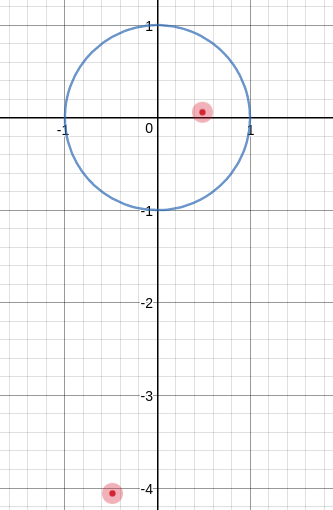
\includegraphics[width=0.3\textwidth]{roots1}
\end{wrapfigure}

 \[\begin{array}{ccc}
 p(S) = \begin{bmatrix} -2i & 4i \\0 &  -2i \end{bmatrix}, & \adj{p}(S) = \begin{bmatrix} 2i & 0 \\-4i  & 2i \end{bmatrix}, &\adj{p}(S) p(S) = \begin{bmatrix} 20 & -8 \\ -8 & 4 \end{bmatrix} \\
 q(S) = \begin{bmatrix} 1 & 4 \\0 & 1 \end{bmatrix}, & \adj{q}(S) =\begin{bmatrix}1 & 0 \\4 & 1 \end{bmatrix}, &\adj{q}(S) q(S) = \begin{bmatrix} 17 & 4 \\ 4 & 1 \end{bmatrix}
\end{array}\]

We get matrix \(H\) as 
\[H = \adj{q}(S) q(S) - \adj{p}(S) p(S) = \begin{bmatrix} -3 & 12 \\ 12 & -3 \end{bmatrix} = 3 \begin{bmatrix} -1 & 4 \\ 4 & -1 \end{bmatrix}\]

The eigenvalues of this matrix are \(-5\) and \(3\). Since one eigenvalue is positive and one is negative, by Schur-Cohn theorem, it means that the polynomial has one root inside the unit circle and one root outside the unit circle. Indeed when the roots are plotted, this result is verified:
%Plot the roots

\clearpage
\section{Conclusion}

The algorithm described above was to determine the location of roots with respect to the unit circle. It can be modified to find the location of roots with respect to a circle of any radius about the origin. To find the number of roots of \(p(z)\) inside a circle of radius \(r\), repeat the above Schur Cohn theorem but with the polynomial \(p(\frac{z}{r})\) instead. This algorithm can be even used to find the number in one half plane of \(\mathbb{C}\).

This method fails when the polynomial has one or more roots on the circle, or if there is a conjugate pair of roots. \(H\) becomes singular and the algorithm fails.  To avoid this, compute the eigenvalues at a circle of a different radius. More workarounds are presented in these papers: Modified versions of this algorithm exist, which are faster but only state if all the roots are within the unit circle or not. 
% Refer to paper S C theorem revisited.

This algorithm has a wide range of applications such as control theory, optimization and digital systems processing, where it is required that all the roots lie in a stability radius of a given point.
\section*{References}


\end{document}